Firstly, it is easy find that cyclopentadienyl radical belongs to the point group $\mathscr{D}_{\rm 5h}$. However, it has only 5 $\pi$-electrons. Just $\mathscr{D}_{\rm 5}$ is good enough and its character table is shown in \Tableref{tab:chatab_3}.
		\begin{center}
		\setlength{\abovecaptionskip}{0em}
		\captionof{table}{The character table for the $\mathscr{D}_{\rm 5}$ point group. Here, $\gamma = \frac{2\pi}{5}$.}\label{tab:chatab_4}
		\begin{tabular}{ccccc}\hline
	$\mathscr{D}_{\rm 5}$ & $E$ & $2C_5$ &	$2C^2_5$	& $5C^\prime_2$ \\ \hline
			$A_1$	&	1	&	1	&	1	&	1	\\
			$A_2$	&	1	&	1	&	1	&	-1	\\
			$E_1$ 	&	2	&$2\cos\gamma$	&	$2\cos2\gamma$	&	0	\\
			$E_2$ 	&	2	&$2\cos2\gamma$	&	$2\cos\gamma$	&	0	\\ \hline
		\end{tabular}
		\end{center}
		
		Secondly, we mark all carbon atoms as follows.
		\begin{center}
		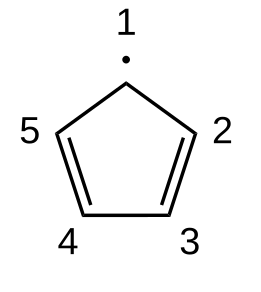
\includegraphics[scale=1.0]{./structures/exercise_1/cyclopentadienyl_radical/0.png}
		\setlength{\abovecaptionskip}{-0.3em}
		\captionof{figure}{The order of carbon atoms in cyclopentadienyl radical.}
		\setlength{\belowcaptionskip}{-0.8em}
		\end{center}				

		For $\pi$-electron atomic orbitals' representation $\Gamma^{\rm AO}$, its following characters is listed below.
		\begin{center}
		\setlength{\abovecaptionskip}{-0.3em}
		\captionof{table}{The character of the $\pi$-electron atomic orbitals' representation $\Gamma^{\rm AO}$.}
		\begin{tabular}{ccccc}\hline
	$\mathscr{D}_{\rm 5}$	& $E$ & $2C_5$ &	$2C^2_5$	& $5C^\prime_2$ \\ \hline
	$\chi^{\AO}(C_i)$	&	5	&	0	&	0	&	-1	\\ \hline
		\end{tabular}\vspace*{-0.5em}
		\end{center}
		Relevant reduction coefficients are
		\begin{equation*}
		a_1 = 0, \quad a_2 = 1, \quad e_1 = 1, \quad e_2 = 1,
		\end{equation*}
		which equal to
		\begin{equation*}
			\Gamma^{\AO} = \Gamma^{A_2} \oplus \Gamma^{E_1} \oplus \Gamma^{E_2}.
		\end{equation*}
		
		\begin{center}
		\begin{tabular}{ccccccccccc}\hline
	$\mathscr{D}_{\rm 5}$ & $E$ & $C^1_5$ & $C^2_5$ & $C^3_5$	&	$C^4_5$	&	$C^\prime_{2,1}$	&	$C^\prime_{2,2}$ &	$C^\prime_{2,3}$	&	$C^\prime_{2,4}$	&	$C^\prime_{2,5}$	\\ \hline
			$\phi_1$	&	$\phi_1$	&	$\phi_2$	&	$\phi_3$	&	$\phi_4$	&	$\phi_5$	&	$-\phi_1$	&	$-\phi_3$	&	$-\phi_5$	&	$-\phi_2$	&	$-\phi_4$	\\
			$\phi_2$	&	$\phi_2$	&	$\phi_3$	&	$\phi_4$	&	$\phi_5$	&	$\phi_1$	&	$-\phi_5$	&	$-\phi_2$	&	$-\phi_4$	&	$-\phi_1$	&	$-\phi_3$	\\ \hline
		\end{tabular}
		\end{center}
		
		For the irreducible representation $\Gamma^{A_2}$, the only basis function is
		\begin{align*}
			P^{A_2}\phi_1 &= \sum_{R} \chi^{A_2}(R) O_R \phi_1 = 2(\phi_1 + \phi_2 + \phi_3 + \phi_4 + \phi_5).
		\end{align*}
		It can be normalized to
		\begin{equation}
			\phi^\prime_1 = \frac{1}{\sqrt{5}}(\phi_1 + \phi_2 + \phi_3 + \phi_4 + \phi_5).
		\end{equation}
		
		Then, the effective Hamiltonian for $\pi$ electrons is
		\begin{equation*}
			H^\prime = ( \alpha + 2\beta ).		
		\end{equation*}
		
		In another words, its only eigenvalue is $\alpha + 2\beta$, with eigenfunction $\Phi^\pi_1 = \phi^\prime_1$.
		
		In conclusion, for the irreducible representation $\Gamma^{A_2}$, relevant results are listed below.
		
		\begin{center}
		\setlength{\abovecaptionskip}{0em}
		\captionof{table}{The H{\"u}ckel MOs in the irreducible representation $\Gamma^{A_2}$ of cyclopentadienyl radical.}
		\begin{tabular}{ccc}\hline
		  order	&	eigenvalue		& 	eigenfunction	\\ \hline
			1	&$\alpha+2\beta$& 	$0.4472\phi_1 + 0.4472 \phi_2 + 0.4472 \phi_3 + 0.4472 \phi_4 + 0.4472 \phi_5$ \\ \hline
		\end{tabular}
		\end{center}
		
		For the irreducible representation $\Gamma^{E_1}$, the only two basis functions are
		\begin{align*}
			P^{E_1}\phi_1 &= \sum_{R} \chi^{E_1}(R) O_R \phi_1 = 2\phi_1 + \frac{\sqrt{5}-1}{2}(\phi_2 + \phi_5) - \frac{\sqrt{5}+1}{2}(\phi_3 + \phi_4). \\
			P^{E_1}\phi_2 &= \sum_{R} \chi^{E_1}(R) O_R \phi_2 = 2\phi_2 + \frac{\sqrt{5}-1}{2}(\phi_1 + \phi_3) - \frac{\sqrt{5}+1}{2}(\phi_4 + \phi_5).
		\end{align*}
		They can be normalized to
		\begin{align*}
			\phi^\prime_2 &= \sqrt{\frac{1}{10}} P^{E_1}\phi_1 = \sqrt{ \frac{2}{5} }\phi_1 + \frac{\sqrt{5}-1}{2\sqrt{10}}(\phi_2+\phi_5) - \frac{\sqrt{5}+1}{2\sqrt{10}}(\phi_3+\phi_4) \\
			&= \sqrt{ \frac{2}{5} } \left[ \phi_1 + \phi_2 \cos\gamma + \phi_3\cos2\gamma + \phi_4\cos2\gamma + \phi_5\cos\gamma \right], \\
			\phi^\prime_3 &= \sqrt{\frac{1}{10}} P^{E_1}\phi_2 = \sqrt{ \frac{2}{5} }\phi_2 + \frac{\sqrt{5}-1}{2\sqrt{10}}(\phi_1+\phi_3) - \frac{\sqrt{5}+1}{2\sqrt{10}}(\phi_4+\phi_5) \\
			&= \sqrt{ \frac{2}{5} } \left[ \phi_1\cos\gamma + \phi_2  + \phi_3\cos\gamma + \phi_4\cos2\gamma + \phi_5\cos2\gamma \right].
		\end{align*}
		However, they are not mutually orthogonal! We have to orthogonalize $\phi^\prime_2$ and $\phi^\prime_3$,
		\begin{align*}
			\phi^\prime_2 + \phi^\prime_3 &= \sqrt{ \frac{2}{5} } \left[ (\phi_1+\phi_2) (1+\cos\gamma) + (\phi_3+\phi_5) (\cos\gamma + \cos 2\gamma) + 2\phi_4\cos2\gamma \right] \\
			&= \sqrt{ \frac{2}{5} } \left[ \frac{3+\sqrt{5}}{4}(\phi_1 + \phi_2) - \frac{1}{2} (\phi_3 + \phi_5) - \frac{ \sqrt{5}+1 }{2} \Phi_4 \right] , \\
			\phi^\prime_2 - \phi^\prime_3 &= \sqrt{ \frac{2}{5} } \left[ (\phi_1-\phi_2) (1-\cos\gamma) + (\phi_3-\phi_5) (\cos2\gamma - \cos\gamma) \right] \\
			&=\sqrt{ \frac{2}{5} } \left[ \frac{ 5-\sqrt{5} }{4} (\phi_1 - \phi_2) - \frac{ \sqrt{5} }{2} (\phi_3 - \phi_5) \right].
		\end{align*}
		and then normalize them. Their sum of squares of coefficients are
		\begin{align*}
			\sum_{k=1}^5 c^2_{2,k} &= \frac{3+\sqrt{5}}{2}, \\
			\sum_{k=1}^5 c^2_{3,k} &= \frac{5-\sqrt{5}}{2},
		\end{align*}
		and then
		\begin{align*}
			\phi^{\prime\prime}_2 &= \sqrt{ \frac{2}{3+\sqrt{5}} } \left[ \phi^\prime_2 + \phi^\prime_3 \right] = \frac{2}{ \sqrt{5(3+\sqrt{5})} } \left[ \frac{3+\sqrt{5}}{4}(\phi_1 + \phi_2) - \frac{1}{2} (\phi_3 + \phi_5) - \frac{ \sqrt{5}+1 }{2} \Phi_4 \right]\\
			&= \frac{ \sqrt{3+\sqrt{5}} }{2\sqrt{5}}(\phi_1 + \phi_2) - \frac{1}{ \sqrt{ 5(3+\sqrt{5}) } } (\phi_3 + \phi_5) - \frac{ 1+\sqrt{5} }{ \sqrt{ 5(3+\sqrt{5}) } } \phi_4 \\
			&\approx 0.5117 \phi_1 + 0.5117 \phi_2 -0.1954 \phi_3 -0.6325\phi_4 -0.1954 \phi_5 , \\
			\phi^{\prime\prime}_3 &= \sqrt{ \frac{2}{5-\sqrt{5}} } \left[ \phi^\prime_2 - \phi^\prime_3 \right] = \frac{2}{ \sqrt{5(5-\sqrt{5})} }\left[ \frac{ 5-\sqrt{5} }{4} (\phi_1 - \phi_2) - \frac{ \sqrt{5} }{2} (\phi_3 - \phi_5) \right] \\
			&= \frac{ \sqrt{ 5-\sqrt{5} } }{ 2\sqrt{5} } (\phi_1 - \phi_2) - \frac{ 1 }{ \sqrt{ 5-\sqrt{5} } }(\phi_3 - \phi_5) \\
			&\approx 0.3717 \phi_1 - 0.3717 \phi_2 - 0.6015\phi_3 + 0.6015 \phi_5.
		\end{align*}
		
		Then, the effective Hamiltonian for $\pi$ electrons is
		\begin{equation*}
			H^\prime = \begin{pmatrix}
				\alpha + \frac{ \sqrt{5}-1 }{2}\beta & 0 \\
				0 & \alpha + \frac{ \sqrt{5}-1 }{2}\beta
			\end{pmatrix} \approx
			\begin{pmatrix}
				\alpha + 0.618 \beta & 0 \\ 0 & \alpha + 0.618 \beta
			\end{pmatrix}				,
		\end{equation*}
		
		In another words, it has only one two-fold eigenvalue $\alpha + \frac{ \sqrt{5}-1 }{2} \beta\approx \alpha + 0.618 \beta$, with two mutually orthogonal eigenfunctions $\Phi^\pi_2 = \phi^{\prime\prime}_2$, $\Phi^\pi_3 = \phi^{\prime\prime}_3$.
		
		In conclusion, for the irreducible representation $\Gamma^{E_1}$, relevant results are listed below.
		
		\begin{center}
		\setlength{\abovecaptionskip}{0em}
		\captionof{table}{The H{\"u}ckel MOs in the irreducible representation $\Gamma^{E_1}$ of cyclopentadienyl radical.}
		\begin{tabular}{ccc}\hline
		  order	&	eigenvalue		& 	eigenfunction	\\ \hline
			1	&$\alpha+0.618\beta$& 	$0.5117\phi_1 + 0.5117 \phi_2 -0.1954 \phi_3 -0.6325 \phi_4 -0.1954 \phi_5$ \\
			2	&$\alpha+0.618\beta$& 	$0.3717\phi_1 - 0.3717 \phi_2 -0.6015 \phi_3 +0.0000 \phi_4 +0.6015 \phi_5$ \\
			 \hline
		\end{tabular}
		\end{center}
		
		For the irreducible representation $\Gamma^{E_2}$, the only two basis functions are
		\begin{align*}
			P^{E_2}\phi_1 &= \sum_{R} \chi^{E_2}(R) O_R \phi_1 = 2\phi_1 - \frac{\sqrt{5}+1}{2}(\phi_2 + \phi_5) + \frac{\sqrt{5}-1}{2}(\phi_3 + \phi_4). \\
			P^{E_2}\phi_2 &= \sum_{R} \chi^{E_2}(R) O_R \phi_2 = 2\phi_2 - \frac{\sqrt{5}+1}{2}(\phi_1 + \phi_3) + \frac{\sqrt{5}-1}{2}(\phi_4 + \phi_5).
		\end{align*}
		They can be normalized to
		\begin{align*}
			\phi^\prime_4 &= \sqrt{\frac{1}{10}} P^{E_1}\phi_1 = \sqrt{ \frac{2}{5} }\phi_1 - \frac{\sqrt{5}+1}{2\sqrt{10}}(\phi_2+\phi_5) + \frac{\sqrt{5}-1}{2\sqrt{10}}(\phi_3+\phi_4) \\
			&= \sqrt{ \frac{2}{5} } \left[ \phi_1 + \phi_2 \cos2\gamma + \phi_3\cos\gamma + \phi_4\cos\gamma + \phi_5\cos2\gamma \right], \\
			\phi^\prime_5 &= \sqrt{\frac{1}{10}} P^{E_1}\phi_2 = \sqrt{ \frac{2}{5} }\phi_2 - \frac{\sqrt{5}+1}{2\sqrt{10}}(\phi_1+\phi_3) - \frac{\sqrt{5}-1}{2\sqrt{10}}(\phi_4+\phi_5) \\
			&= \sqrt{ \frac{2}{5} } \left[ \phi_1\cos2\gamma + \phi_2  + \phi_3\cos2\gamma + \phi_4\cos\gamma + \phi_5\cos\gamma \right].
		\end{align*}
		However, they are not mutually orthogonal! We have to orthogonalize $\phi^\prime_4$ and $\phi^\prime_5$,
		\begin{align*}
			\phi^\prime_4 + \phi^\prime_5 &= \sqrt{ \frac{2}{5} } \left[ (\phi_1+\phi_2) (1+\cos2\gamma) + (\phi_3+\phi_5) (\cos\gamma + \cos 2\gamma) + 2\phi_4\cos\gamma \right] \\
			&= \sqrt{ \frac{2}{5} } \left[ \frac{3-\sqrt{5}}{4}(\phi_1 + \phi_2) - \frac{1}{2} (\phi_3 + \phi_5) + \frac{ \sqrt{5}-1 }{2} \Phi_4 \right] , \\
			\phi^\prime_4 - \phi^\prime_5 &= \sqrt{ \frac{2}{5} } \left[ (\phi_1-\phi_2) (1-\cos2\gamma) + (\phi_3-\phi_5) (\cos\gamma - \cos2\gamma) \right] \\
			&=\sqrt{ \frac{2}{5} } \left[ \frac{ 5+\sqrt{5} }{4} (\phi_1 - \phi_2) + \frac{ \sqrt{5} }{2} (\phi_3 - \phi_5) \right].
		\end{align*}
		and then normalize them. Their sum of squares of coefficients are
		\begin{align*}
			\sum_{k=1}^5 c^2_{4,k} &= \frac{3-\sqrt{5}}{2}, \\
			\sum_{k=1}^5 c^2_{5,k} &= \frac{5+\sqrt{5}}{2},
		\end{align*}
		and then
		\begin{align*}
			\phi^{\prime\prime}_4 &= \sqrt{ \frac{2}{3-\sqrt{5}} } \left[ \phi^\prime_4 + \phi^\prime_5 \right] = \frac{2}{ \sqrt{5(3-\sqrt{5})} } \left[ \frac{3-\sqrt{5}}{4}(\phi_1 + \phi_2) - \frac{1}{2} (\phi_3 + \phi_5) + \frac{ \sqrt{5}-1 }{2} \Phi_4 \right]\\
			&= \frac{ \sqrt{3-\sqrt{5}} }{2\sqrt{5}}(\phi_1 + \phi_2) - \frac{1}{ \sqrt{ 5(3-\sqrt{5}) } } (\phi_3 + \phi_5) + \frac{ \sqrt{5}-1 }{ \sqrt{ 5(3-\sqrt{5}) } } \phi_4 \\
			&\approx 0.1954 \phi_1 + 0.1954 \phi_2 - 0.5117 \phi_3 +0.6325\phi_4 -0.5117 \phi_5 , \\
			\phi^{\prime\prime}_5 &= \sqrt{ \frac{2}{5+\sqrt{5}} } \left[ \phi^\prime_4 - \phi^\prime_5 \right] = \frac{2}{ \sqrt{5(5+\sqrt{5})} }\left[ \frac{ 5+\sqrt{5} }{4} (\phi_1 - \phi_2) + \frac{ \sqrt{5} }{2} (\phi_3 - \phi_5) \right] \\
			&= \frac{ \sqrt{ 5+\sqrt{5} } }{ 2\sqrt{5} } (\phi_1 - \phi_2) + \frac{ 1 }{ \sqrt{ 5+\sqrt{5} } }(\phi_3 - \phi_5) \\
			&\approx 0.6015 \phi_1 - 0.6015 \phi_2 + 0.3717\phi_3 -0.3717 \phi_5.
		\end{align*}
		
		Then, the effective Hamiltonian for $\pi$ electrons is
		\begin{equation*}
			H^\prime = \begin{pmatrix}
				\alpha - \frac{ \sqrt{5}+1 }{2}\beta & 0 \\
				0 & \alpha - \frac{ \sqrt{5}+1 }{2}\beta
			\end{pmatrix} \approx
			\begin{pmatrix}
				\alpha - 1.618 \beta & 0 \\ 0 & \alpha - 1.618 \beta
			\end{pmatrix}				,
		\end{equation*}
		
		In another words, it has only one two-fold eigenvalue $\alpha + \frac{ \sqrt{5}-1 }{2} \beta\approx \alpha - 1.618 \beta$, with two mutually orthogonal eigenfunctions $\Phi^\pi_4 = \phi^{\prime\prime}_4$, $\Phi^\pi_5 = \phi^{\prime\prime}_5$.
		
		In conclusion, for the irreducible representation $\Gamma^{E_2}$, relevant results are listed below.
		
		\begin{center}
		\setlength{\abovecaptionskip}{0em}
		\captionof{table}{The H{\"u}ckel MOs in the irreducible representation $\Gamma^{E_2}$ of cyclopentadienyl radical.}
		\begin{tabular}{ccc}\hline
		  order	&	eigenvalue		& 	eigenfunction	\\ \hline
			1	&$\alpha-1.618\beta$& 	$0.1954\phi_1 + 0.1954 \phi_2 -0.5117 \phi_3 +0.6325 \phi_4 -0.5117 \phi_5$ \\
			2	&$\alpha-1.618\beta$& 	$0.6015\phi_1 - 0.6015 \phi_2 +0.3717 \phi_3 +0.0000 \phi_4 -0.3717 \phi_5$ \\	 \hline
		\end{tabular}
		\end{center}
		
		Now, we have obtained all results, which are shown as following.
		
		\begin{center}
		\setlength{\abovecaptionskip}{-0.5em}
		\captionof{table}{The H{\"u}ckel MOs in all irreducible representations of cyclopentadienyl radical.}
		\begin{tabular}{cccccccc}\hline
		order 	& orbital energy & irrep & $c_1$ & $c_2$ & $c_3$ &$c_4$ &	$c_5$	\\ \hline
			1	&	$\alpha+2.000\beta$	&	$A_2$	&	0.4472	&	0.4472	&	0.4472	&	0.4472	&	0.4472	\\
			2	&	$\alpha+0.618\beta$	&	$E_1$	&	0.5117	&	0.5117	&	-0.1954	&	-0.6325	&	-0.1954	\\
			3	&	$\alpha+0.618\beta$	&	$E_1$	&	0.3717	&	-0.3717	&	-0.6015	&	0.0000	&	0.6015	\\
			4	&	$\alpha-1.618\beta$	&	$E_2$	&	0.1954	&	0.1954	&	-0.5117	&	0.6325	&	-0.5117	\\
			5	&	$\alpha-1.618\beta$	&	$E_2$	&	0.6015	&	-0.6015	&	0.3717	&	0.0000	&	-0.3717	\\ \hline
		\end{tabular}
		\end{center}
		
		Besides, their phase diagrams have been painted in \Figref{fig:phase_diagram_4}.
		
		\begin{center}
		\begin{tabular}{ccccc}
			\begin{minipage}[t]{0.17\linewidth}
			\centering
			\setlength{\abovecaptionskip}{0.5em}
			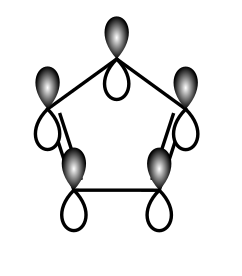
\includegraphics[scale=1]{./structures/exercise_1/cyclopentadienyl_radical/1.png}
			\captionof*{figure}{$\varepsilon = \alpha + 2.000\beta$}
			\end{minipage} & 
			\begin{minipage}[t]{0.17\linewidth}
			\setlength{\abovecaptionskip}{0.5em}\hspace*{0.2em}
			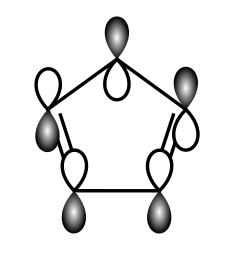
\includegraphics[scale=1]{./structures/exercise_1/cyclopentadienyl_radical/2.png}
			\captionof*{figure}{$\varepsilon = \alpha + 0.618\beta$}
			\end{minipage} &
			\begin{minipage}[t]{0.18\linewidth}
			\centering
			\setlength{\abovecaptionskip}{0.5em}
			\hspace*{-0.2em}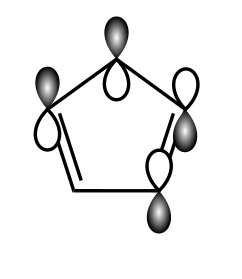
\includegraphics[scale=1]{./structures/exercise_1/cyclopentadienyl_radical/3.png}
			\captionof*{figure}{$\varepsilon = \alpha + 0.000\beta$}
			\end{minipage} & 
			\begin{minipage}[t]{0.18\linewidth}
			\setlength{\abovecaptionskip}{0.5em}\hspace*{0.5em}
			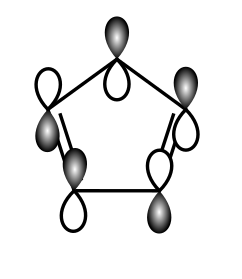
\includegraphics[scale=1]{./structures/exercise_1/cyclopentadienyl_radical/4.png}
			\captionof*{figure}{$\varepsilon = \alpha - 2.000\beta$}
			\end{minipage}
			\begin{minipage}[t]{0.18\linewidth}
			\setlength{\abovecaptionskip}{0.5em}\hspace*{0.5em}
			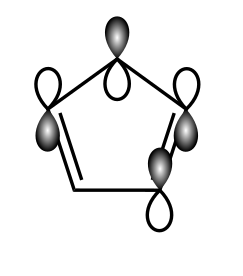
\includegraphics[scale=1]{./structures/exercise_1/cyclopentadienyl_radical/5.png}
			\captionof*{figure}{$\varepsilon = \alpha - 2.000\beta$}
			\end{minipage}
		\end{tabular}				
		\captionof{figure}{Phase diagrams of these H{\"u}ckel MOs of cyclopentadienyl radical. Black bubbles mean plus phase while white ones mean minus phase. The color is used just for determining relative phase.}\label{fig:phase_diagram_4}
		\end{center}
		
		In the end, we conclude that for cyclopentadienyl radical, its ground state $\pi$-electron configuration is $(a_2)^2(e_1)^3$ and its delocalization energy is $2 \times 2.000 \beta + 3 \times 0.618 \beta - 5 \times 1.000 \beta = 0.854 \beta$, much larger than {\it trans}-1,3-butadiene ($0.472\beta$) but also much smaller than benzene ($2.000\beta$). 